% Appendix A

\chapter{I2C Bus Transactions}
\label{AppendixA}
\lhead{Appendix A. \emph{I2C Transactions}}





\section{Basics of I2C}
The I2C is a is a synchronous serial communication protocol that uses 2 wires, SCL (serial clock) and SDA (serial data), hence also called the “2-wire” interface. It transfers data in bytes, where the LSB of the starting bit indicates a read or write operation, so I2C devices mostly have a 7-bit address. The address byte is followed by the pointer byte, that tell the device which register is to be accessed. The I2C is a network interface, so there may be multiple masters and multiple slaves. Buffers are marked with a start and stop bit, and each buffer is 8-bit long.
\begin{figure}[htbp]
	\centering
		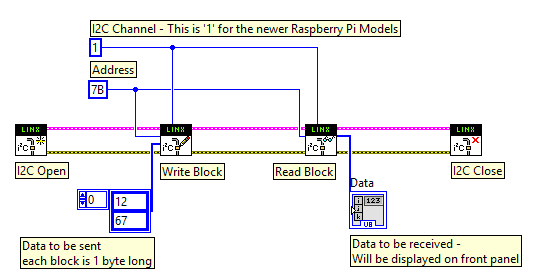
\includegraphics[width = 5in]{./Figures/I2Cexample.png}
		\rule{35em}{0.5pt}
	\caption{I2C example using LabVIEW}
	\label{fig:I2C example using LabVIEW}
\end{figure}
Here is a sample VI of I2C transaction in LabVIEW. There is no need of sending a 0(read) or 1(write) in LabVIEW as the blocks for read and write command are separate and do this automatically. This problem was faced at the beginning as we were sending 0s and 1s and hence no output was received.

\section{ADS1115}
The ADS1115 is a 16-bit ADC with 4 channels for analog input. It has a variable sensitivity and a variable sampling rate, that can be adjusted using the control register. The control register also selects the ADC channel from which we want to receive data. One channel can be read at a time. Since it is a 16-bit ADC, 2 bytes are to be read for a single channel. Here is an example transaction

\begin{figure}[htbp]
	\centering
		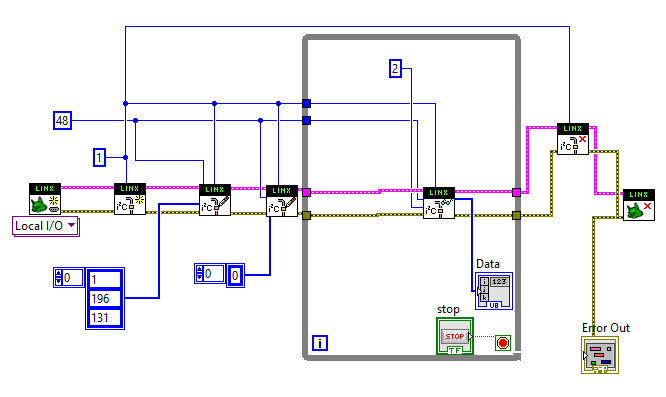
\includegraphics[width = 5in]{./Figures/ADS-1115.png}
		\rule{35em}{0.5pt}
	\caption{ADS1115 example using LabVIEW}
	\label{fig:ADS1115 example using LabVIEW}
\end{figure}

This module has only two possible values for pointer. Writing a 1 in 1st byte of buffer tells the module that we want to configure the control registers, and then write two bytes for the control registers. Writing a 0 tells it that we want to read, so writing a zero is followed by a read command, and it will continue till we write another command. 

\section{PCA9685}
The PCA9685 is a 12-bit, 16 channel PWM driver.	It has a variable PWM frequency that can be adjusted by the pre-scale register. It also has 2 registers for basic configurations such as sleep, open drain, invert, etc. named as MODE1 and MODE2. It also has an ALL-CALL register that sets the same value on all channels. Apart from this, each channel is 12-bit, so we need 2 register per channel, but instead, 4 are available per channel, two for setting the rising edge time, and two for the falling edge time. The registers for rising edge will be set to 0, so the pulse starts at time zero, and now we control the output using the falling edge register, named as LEDx\textunderscore OFF\textunderscore L and LEDx\textunderscore OFF\textunderscore H. Below is an example of the PCA9685 control using LabVIEW, on channel 0, using a slider on the front panel.

\begin{figure}[htbp]
	\centering
		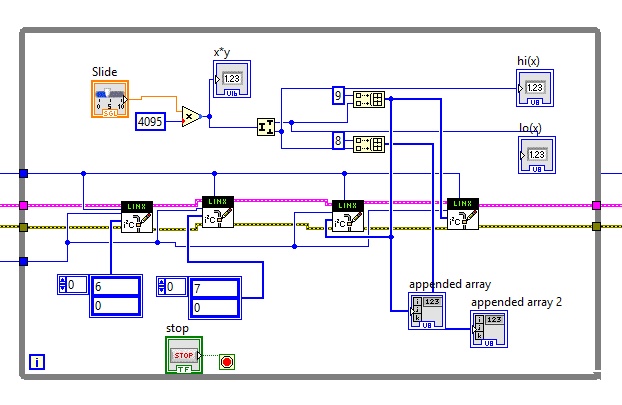
\includegraphics[width = 5in]{./Figures/PCA-9685.png}
		\rule{35em}{0.5pt}
	\caption{PCA9685 example using LabVIEW}
	\label{fig:PCA9685 example using LabVIEW}
\end{figure}



\section{MPU6050}
The MPU6050 is an IMU with a MEMS accelerometer and gyroscope, and contains a 16-bit ADC. It has 6 DOF, i.e. x, y and z for accelerometer and roll, pitch and yaw for gyroscope. The I2C block for MPU-6050 is available in LabVIEW, so we do not need to use the previous method for I2C transactions. In the project, we have used GY-521, which is a breakout board for the MPU-6050. Here is an example VI that extracts raw accelerometer and gyroscope data from the MPU. The brown wire represents a cluster, all the values of gyroscope and accelerometer, and need to be separated using the ‘unbundle’ block in LabVIEW.


\begin{figure}[htbp]
	\centering
		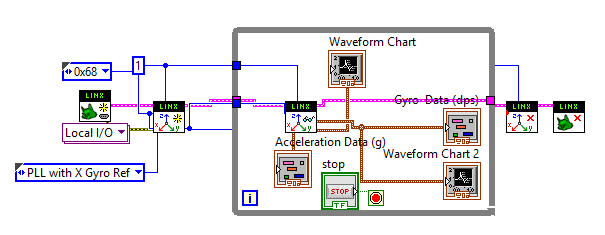
\includegraphics[width = 6in]{./Figures/MPU-6050.png}
		\rule{35em}{0.5pt}
	\caption{MPU6050 example using LabVIEW}
	\label{fig:MPU6050 example using LabVIEW}
\end{figure}